\section{Cinema 4D [M]}
\setauthor{Fabian Maar}
Cinema 4D ist ein professionelles Programm des Unternehmens Maxon zur 3D-Modellierung und Animation. Zum einen ist die Software leicht zu bedienen und zum anderen bietet Maxon eine Vielzahl an Tutorials und Anleitungen. Im Unterschied zu anderen 3D-Programmen wie Autodesk Maya, gelingt es durch Cinema 4D eine geringe und effiziente Lernkurve zu erreichen. Aufgrund der intuitiven Benutzeroberfläche mit vielen Funktionen ist das Programm sowohl für Einsteiger als auch für Profis geeignet. \cite{Cinema4D}

\begin{figure} [h t]
    \centering
    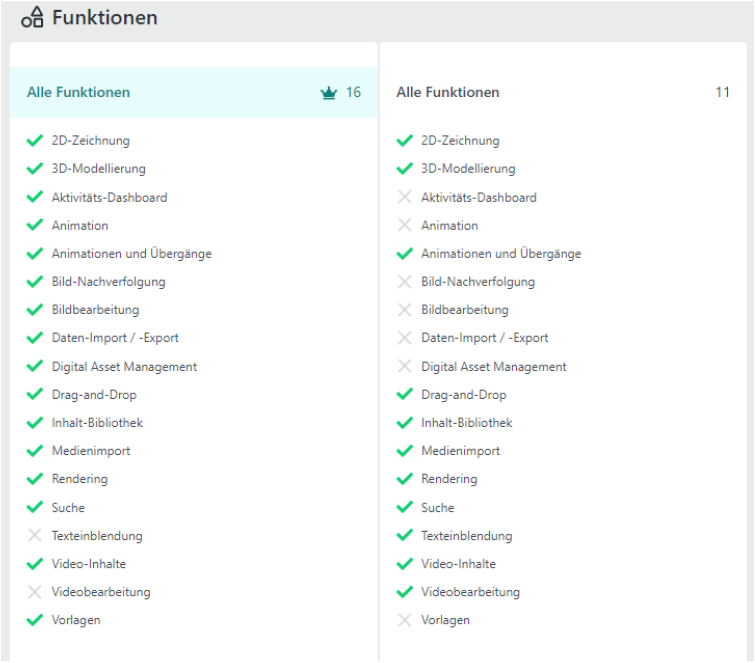
\includegraphics[scale=0.7]{pics/c4d-vs-maya.PNG}
    \caption{Cinema4D vs Maya \cite{C4DvsMaya}}
    \label{fig:tech:front:c4d-vs-maya}
  \end{figure}

Ein weiterer wichtiger Aspekt ist, dass Cinema 4D den Export von GLTF-Files unterstützt. GLTF ist das Dateiformat, das genutzt wird, um ein 3D-Modell in der Three.js Szene zu laden. Da alternative 3D-Programme wie zum Beispiel Blender diese Exportmöglichkeit nicht anbieten, war Cinema 4D die gewählte Option für die 3D-Modellierung.   

\subsection{Modellierung der 3D-Räume in Cinema 4D}
\setauthor{Fabian Maar}

Zu Beginn wird der Grundriss des Raumes gezeichnet. Dies erfolgt durch das Spline-Werkzeug. Hierbei werden 2D-Linien im dreidimensionalen Raum erstellt. Anschließend wird ein Würfel erstellt, der die Höhe und Breite besitzt, die eine Wand haben soll. Da Cinema 4D die Modelle in Zentimeter misst, können diese in realitätsnahen Proportionen modelliert werden. Um den 2D-Grundriss nun als dreidimensionale Wände abzubilden, werden die gezeichneten Splines mit der Form des Würfels als Sweep extrudiert. Das bedeutet, eine 2D-Form wird als schlauchförmiges 3D-Objekt mit den Werten des Würfels erstellt. Nach diesem Vorgang kann schlussendlich der Boden des Raumes hinzugefügt werden. Dazu wird eine Platte in Form des Grundrisses erstellt. 

\begin{figure} [h t]
    \centering
    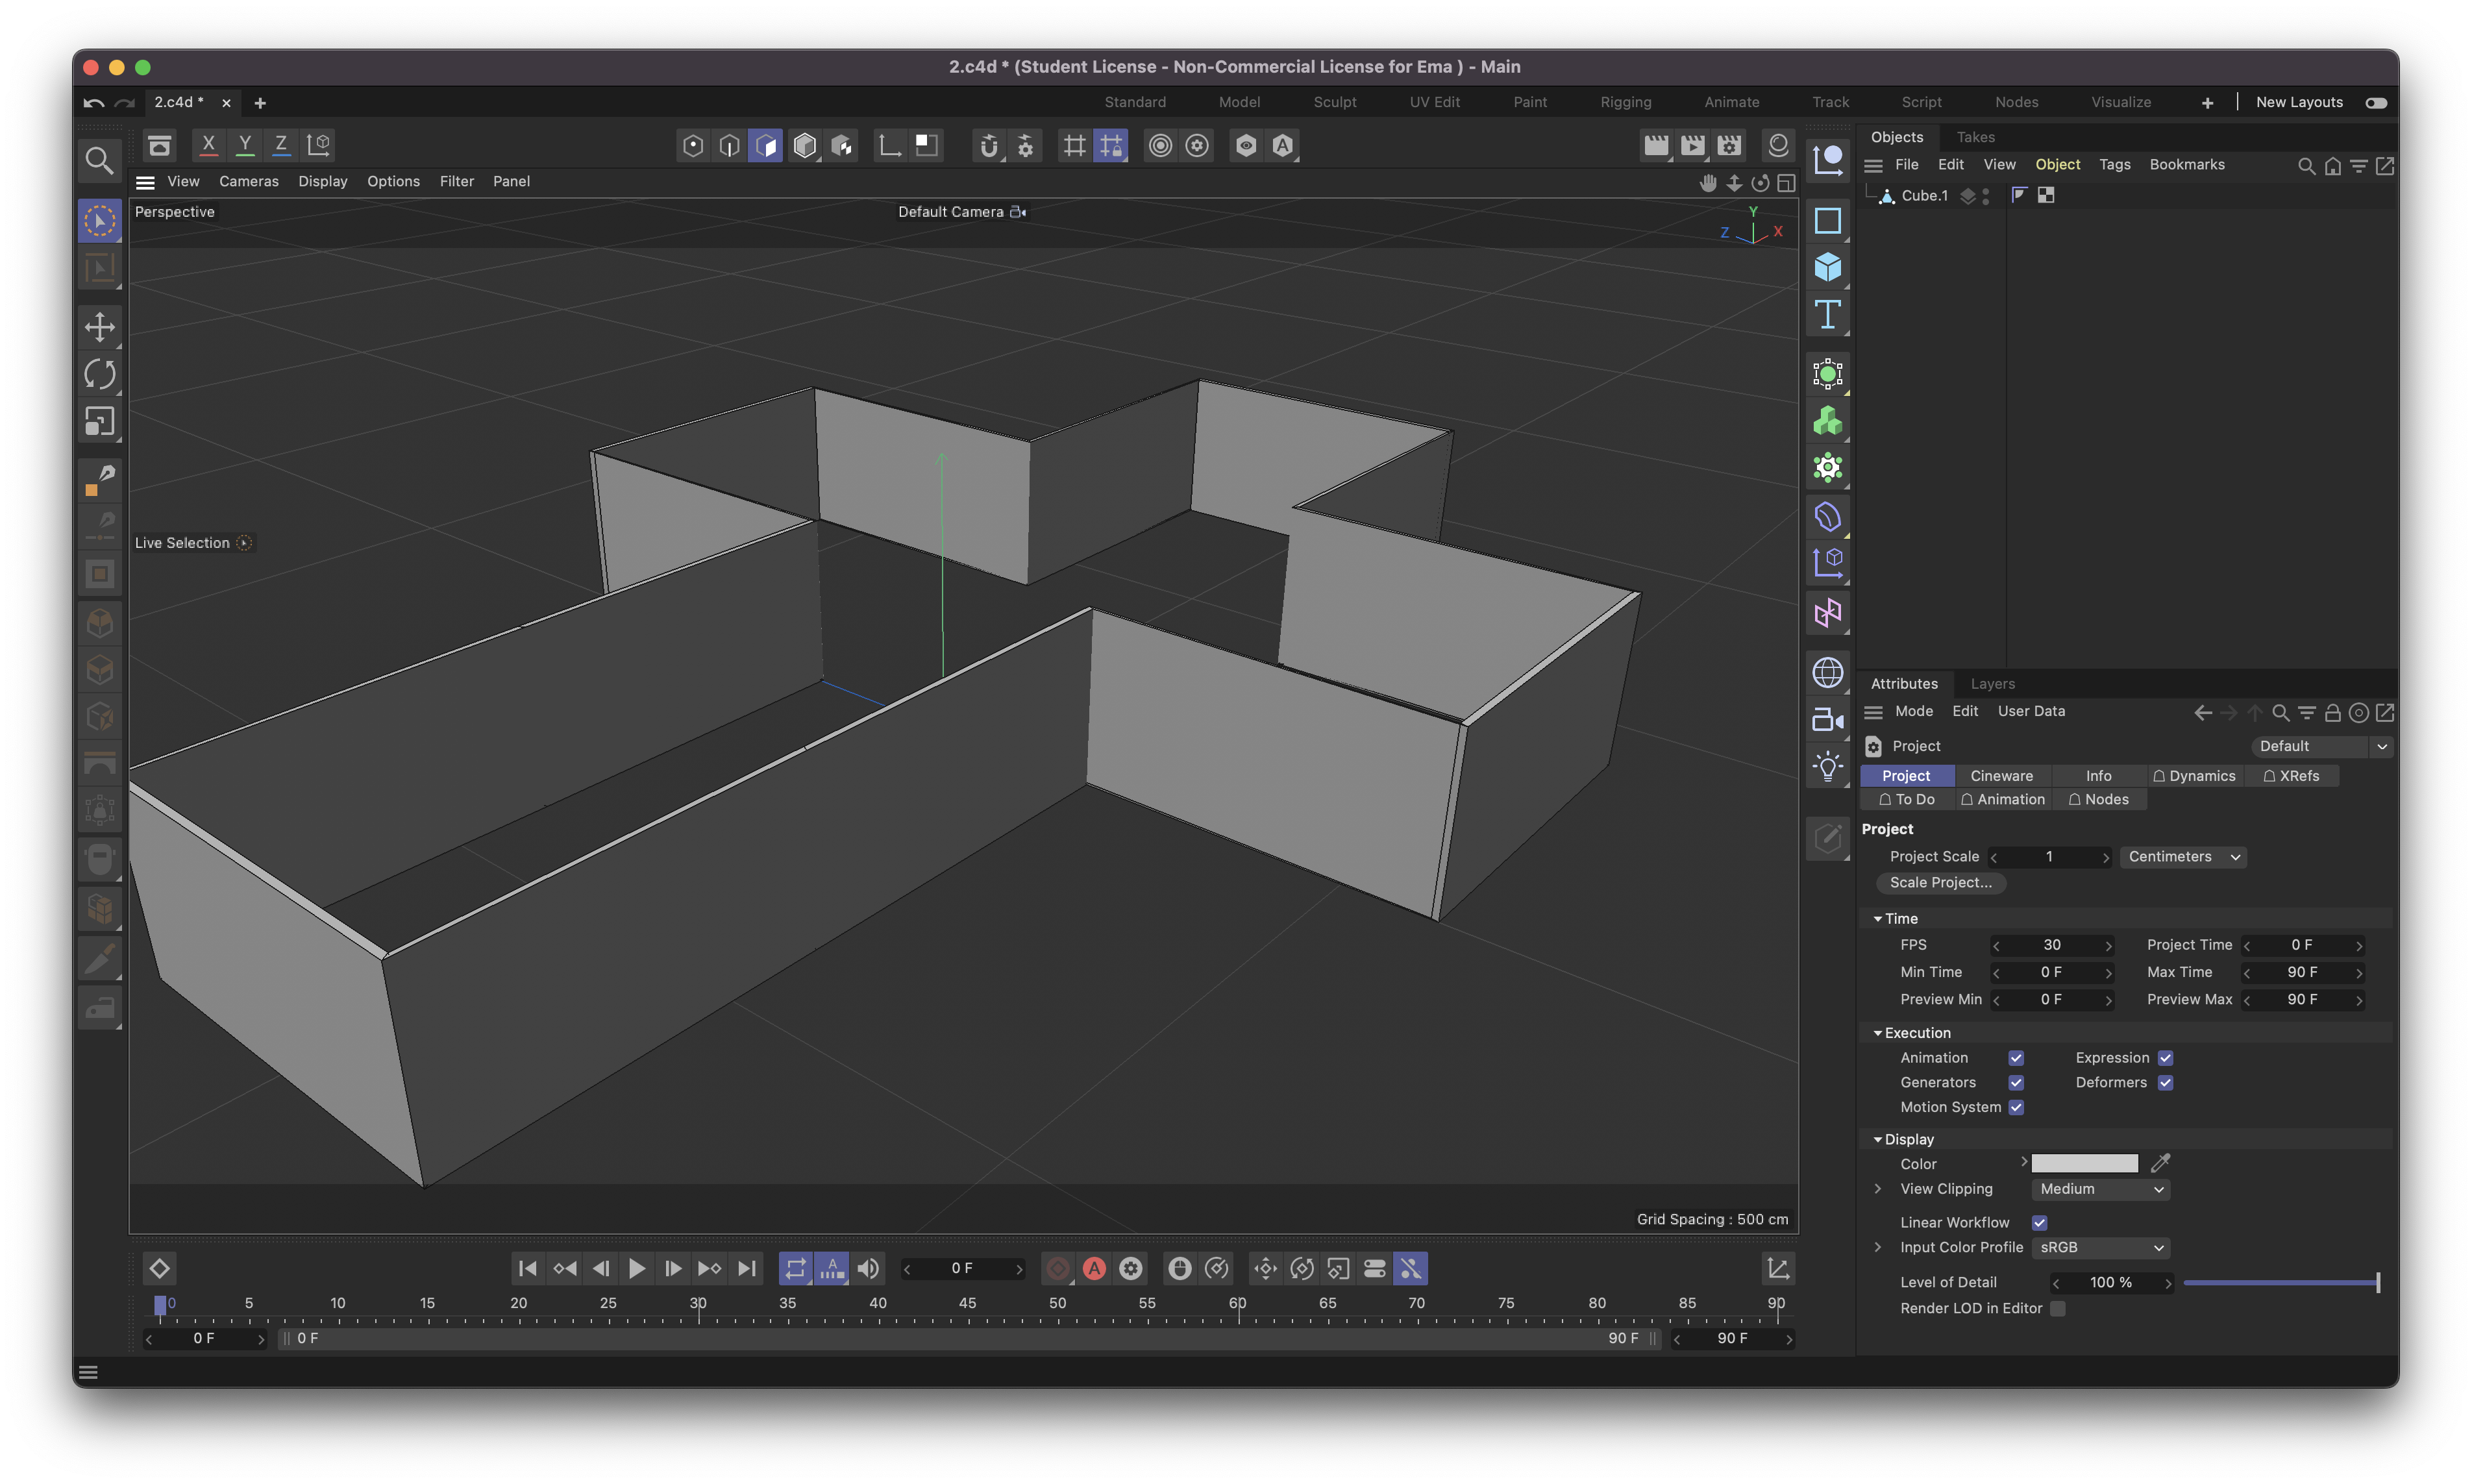
\includegraphics[scale=0.2]{pics/Room-model.png}
    \caption{Modellierung des Raumes in Cinema4D}
    \label{fig:tech:front:room-model}
  \end{figure}



\section{Figma [L]}
\setauthor{Litzlbauer Lorenz}
\label{ch::technologies::figma}
Figma ist ein Programm für die Erstellung und Testung von UI und UX Prototypen. Das Programm ist einsteigerfreundlich, denn es hat eine benutzerfreundliche Oberfläche und es gibt viele Tutorials auf der Webseite und von der Figma Community. Figma ist primär eine Web-Applikation, bietet aber auch eine Desktop-Version für macOS und Windows und eine mobile Version für iOS und Android an. Figma arbeitet mit mehreren Konzepten, um den Designprozess zu vereinfachen:
\paragraph{Kollaboration}
In Figma können mehrere Personen gleichzeitig auf verschiedenen Geräten designen. Es gibt verschiedene Rollen, wie Zuschauer*in, Kritiker*in oder Mitarbeiter*in. Die Möglichkeiten können genutzt werden um einen*einer Kunden*in in den Designprozess zu involvieren und schon früh Feedback auf das Design bekommen zu können.
\paragraph{Plugins}
Figma hat eine große Community, gibt es ein Feature nicht, kann dieses von der Community im PluginStore als Plugin hinzugefügt werden. Ein Plugin ist eine Software-Erweiterung, welche die Fähigkeiten oder die Features eines Softwareprojektes erweitert.

\paragraph{Assets}
Figma arbeitet mit dem Konzept der Assets. Bereits designte Komponenten können als Assets gespeichert werden. Figma legt einen großen Wert auf die Modularität, es können Farben und Pixelgrößen als Variable gespeichert werden, wenn diese sich verändern, verändern sich gleichzeitig die darauf referenzierenden Assets.

\subsection{Auswahl}
Wegen dieser vielen Features und persönlichen Erfahrungen in privaten Projekten bot sich Figma für dieses Projekt als UX/UI-Design- Tool an.